\documentclass[11pt]{article}
\usepackage[utf8]{inputenc}
%\usepackage{eurosym}
\usepackage{eurosym}
\usepackage{graphicx}
\usepackage{libertine}
\usepackage[multiple]{footmisc}
\usepackage{microtype}
\usepackage{enumitem}
\setlist{nosep}
\usepackage[margin=3cm,a4paper]{geometry}
\usepackage[hidelinks,colorlinks]{hyperref}

\title{For Overlay Journals in Mechanics}
%\author{Vincent Acary [Inria Grenoble] and Mathias Legrand [McGill University]}
%\date{}
\begin{document}
\maketitle
\noindent The purpose of this letter is to raise awareness among the communities in Mechanics about epijournal publications. Hyperlinks are given as footnotes.
\section*{Problem}
How is all this possible? Tomorrow, researchers will have to pay in order to publish! The Gold Open Access model with Article Processing Charge (APC) seems to expand rapidly in our community. This publication process uses a business model based on individual articles for which their authors pay fees for publication\footnote{\href{https://en.wikipedia.org/wiki/Article_processing_charge}{Definition of APC on Wikipedia}}.

\section*{Public finances}
This model will have dramatic consequences on universities' and research institutes' budgets, and more generally on public finances. For instance in France, CNRS currently spends about M\EUR{15}/year in library resources, amount that would nicely reach M\EUR{95}/year in case Gold Access with APC becomes the preferred avenue for publishing\footnote{\href{http://www.cnrs.fr/dist/z-outils/documents/Distinfo2/DISTetude_4.pdf}{DIST Etude 2015 assuming that all CNRS authors will pay for their contributions.}}. Similar numbers are provided by McGill's library concerning the subscription to journals and electronic resources\footnote{\href{http://www.mcgill.ca/library/files/library/mcgill_library_and_archives_-_annual_report_2016_0.pdf}{2016 Annual Report, page 13}}. Moreover, the H2020 program promotes open access in the general sense, with or without APC, but has the harmful side-effect if there is no alternative  but to pay under the Gold Open Access policy. The fact that APC are eligible expenses to be listed in proposals of H2020 is a consequence of this ambiguity.
%This situation is not sustainable. 
Some might think that APC represent a minor fraction of research expenses. This is probably true but a publication process free of charges for both authors and readers (Diamond Open Acess Policy\footnote{\href{https://en.wikipedia.org/wiki/Open_access_journal}{Definition of Diamond Access Policy}}) is a viable alternative.

\section*{Open Access, sustainable research and epijournals}
As our colleagues in Mathematics, Computer Science and Human Sciences have already understood\footnote{\href{https://www.cimpa.info/en/node/62}{List of Mathematical Journals that apply a Diamond Open Access policy}}\footnote{\href{https://www.episciences.org/page/journals}{épisciences.org Overlay Journals}}, Overlay Journals (also called epijournals or Diamond Open Access) are the way to go! Overlay journals are purely open access electronic journals solely fed by articles that are deposited on open archives (arXiv, HAL, engrXiv...) and not already published elsewhere. The review procedure, undertaken by the editorial team of the overlay journal together with designated reviewers, is of high quality\footnote{\href{http://discreteanalysisjournal.com/articles and its announcement by Nature https://www.nature.com/news/leading-mathematician-launches-arxiv-overlay-journal-1.18351}{Discussion on the Discrete Analysis Overlay Journal in Mathematics}}. This virtuous framework involves a minimal cost to society and taxpayers while publications (and possibly attendant data) are always openly accessible on the long term. Technical challenges are minimal since appropriate platforms already exist. As an example, the Episciences initiative\footnote{\href{https://www.episciences.org/?lang=en}{épisciences.org Website}} provides technical support for peer-reviewing activities which are supervised by editorial boards. To summarize, epijournals add value to open archives by assigning a scientific caution to the accepted papers. Other benefits of \emph{free} Open Access\footnote{We call ``free Open Access'', a publication model free of charges for both authors and readers or equivalently the Diamond Open Acess Policy} are summarized in Figure~\ref{fig:OA}.
\begin{figure}[ht]\centering%
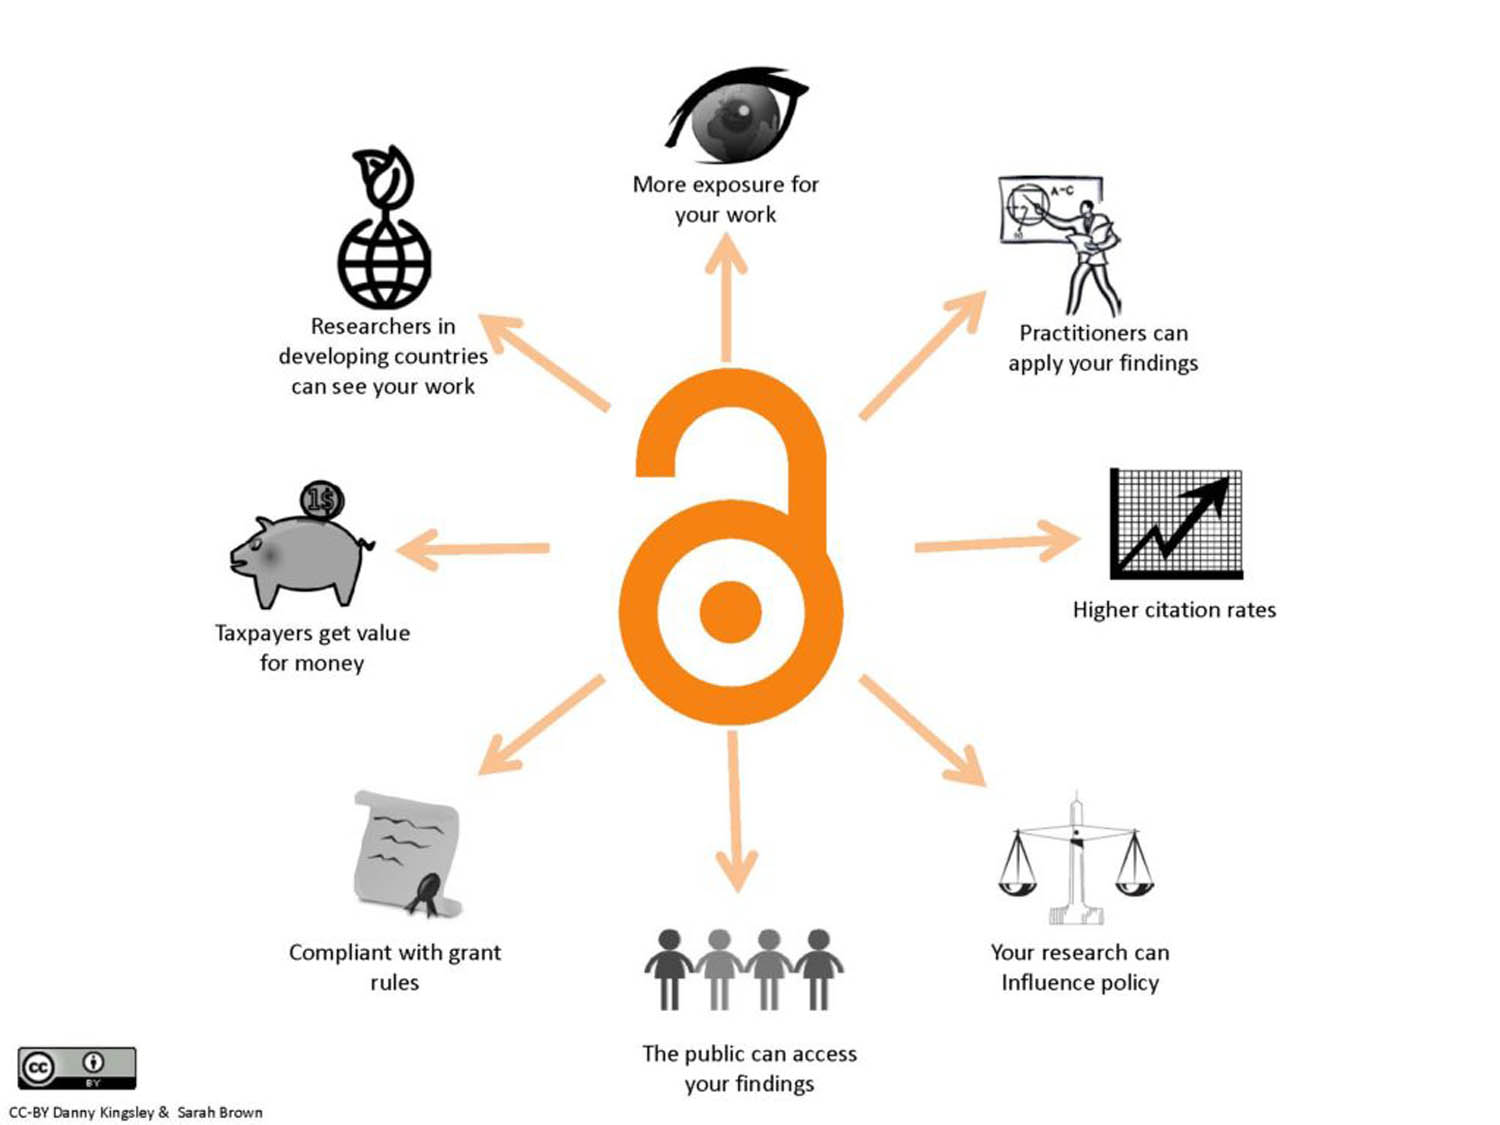
\includegraphics[width=14cm]{OA.jpg}\caption{Benefits of \emph{free} Open Access}\label{fig:OA}
\end{figure}

\section*{And the mechanics community?}
It is now critical that the mechanics community thinks about a full open access model to publish the outcomes of research, and more specifically about the creation of Overlay Journals in various subfields of Mechanics. Lately, this question generated a strong interest as it is witnessed by the fruitful discussion on Loomio, an online tool increasing transparency and inclusion, to reach decisions\footnote{\href{https://www.loomio.org/invitations/aa0a97be9a80ba509623}{Loomio discussion on Overly Journals in Mechanics}}.

\section*{Next steps and questions to the Scholarly Society}
An international editorial team should now be created. It is highly recommended that Scholarly Societies get involved in the creation of Epijournals and blow a wind of change able to completely redraw the arcane of publishing. Also, we would like the point of view of the society on the following questions:
\begin{itemize}
\item Would the Society position itself as a proponent of alternative publication processes based on epijournals?
\item Would the Society be able to support an initiative for creating an epijournal in Mechanics?
\item Could the Society suggest members to the editorial board of the epijournal to be created?
\item Would the Society be willing to help implement the launch of the such a journal by encouraging the submission of papers after international conferences and workshop administered by the society?\\[15pt]
\end{itemize}
On behalf of the Loomio members supporting the creation of Epijournals in Mechanics, \\[10pt]
Vincent Acary, INRIA, France\\
Mathias Legrand, McGill University, Canada
\end{document}

                        
                                
                                        
Also, we would like the point of view of the society on the following questions: 
                                        
• Would the Society position itself as a proponent of alternative publication processes based on epijournals? 
                                        


• Could the Society suggest a list of members to the editorial board and/or scientific comittee for the epijournal? 

• Would the Society encourage  submissions of papers in the frame of international conferences and workshop sponsored by the society? 

• More generally, would the Society be able to support an initiative for creating an epijournal in Mechanics and how? 


We would appreciate a formal answer in the shape of a letter. This point may be planned in the agenda of your next steering committee.
 
This letter has been sent to [list of societies].  All the answers will be publicly available on the following website. 

https://epijournalinmechanics.github.io


%%% Local Variables:
%%% mode: latex
%%% TeX-master: t
%%% End:
